\documentclass{article}
\usepackage[utf8]{inputenc}
\usepackage{geometry}
\usepackage{graphicx}
\usepackage{pgfplots}
\usepackage{amsmath}
\usepackage{amssymb}
\usepackage{amsfonts}
\usepackage{mdframed}
\usepackage{amsthm}
\usepackage{tikz}
\usepackage{multicol}
\usepackage{cancel}
\usepackage{hyperref}

\geometry{a4paper, left=2cm, right=2cm, top=1cm, bottom=2cm}

\pgfplotsset{compat=1.18}
\begin{document}

\begin{minipage}{0.7\textwidth}
    \small \textbf{Fenómenos Colectivos}  \\
    \small {Facultad de Ciencias, Universidad Nacional Autónoma de México} \\
    \small {Profesora: Dra. Catalina Elizabeth Stern Forgach} \\
    \small {Ayudante: M. Tyra Delgadillo Mendoza} \\
    \small {Fecha de entrega: Lunes 11 de febrero del 2024} \\
    \small {Nombre completo: Andrés López González} \\
    \small {Actividad en clase}
\end{minipage}
\hfill
\begin{minipage}{0.12\textwidth}
    
\includegraphics[width=\linewidth]{logo_universidad}
\end{minipage}\\\\

\noindent I. Una masa de hidrógeno gaseoso ocupa un volumen de 230 litros en un tanque a una presión de 1.5 atm y a una temperatura de 35C. Calcular a) ¿Cuántos moles de hidrógeno se tienen? B) A qué masa equivale ese número de moles. \\
\textit{Utilizamos la ecuación de los gases ideales.}
\begin{equation}
    PV = nRT
\end{equation}
\textit{Despejamos el número de moles.}
\begin{equation*}
    n = \frac{PV}{RT} = \frac{1.5atm \cdot 230L}{0.0821 \frac{atm \, L}{K \, mol}\cdot(35+273.15)K} \approx 13.63684 \, \textit{moles de hidrógeno}
\end{equation*}
\textit{Para la masa en gramos ocupamos la siguiente ecuación en donde m es la masa en gramos, n la cantidad de moles y M la masa molar del hidrógeno.}
\begin{equation*}
    m = n \cdot M = 13.63684mol \cdot 1.00797 g/mol \approx 13.74552g
\end{equation*}

\noindent II. En un laboratorio hay 20 moles de un gas ideal que se expanden isotérmicamente. La presión inicial es de 10atm y el volumen de 8 litros. Al final, el volumen es de 40litros. a) ¿Cuál es la presión final?, b) ¿Cuál es la temperatura? \\
\textit{Utilizando la ley de Boyle-Mariotte.}
\begin{equation}
    P_1V_1 = P_2V_2
\end{equation}
\textit{Despejamos la presión final $P_2$.} \\
\begin{equation*}
    P_2 = \frac{P_1V_1}{V_2} = \frac{10atm \cdot 8L}{40L} = 2atm
\end{equation*}
\textit{Dado que es un sistema isotérmico los cálculos son mucho más simples, utilizaremos la ecuación de los gases ideales denotada por (1), en la que aislaremos la temperatura. Nótese que es indiferente usar las presiones y volúmenes iniciales o finales por lo recién visto en la ley de Boyle-Mariotte.}
\begin{equation*}
    T = \frac{PV}{nR} = \frac{P_2V_2}{nR} = \frac{2atm \cdot 40L}{20mol \cdot 0.0821 \frac{atm \, L}{K \, mol}} = 48.72107K
\end{equation*}

\noindent III. En una máquina térmica se emplea vapor de una caldera a 230C para producir trabajo y ceder lo sobrante al medio ambiente que está a 102C. ¿Cuál es la eficiencia? \\
\textit{Utilizamos la ecuación de la eficiencia que involucra la razón entre el foco frío y caliente.}
\begin{equation}
    e = 1 - \frac{T_f}{T_c}
\end{equation}
\textit{Convertimos en grados Kelvin al igual que el primer ejercicio sumando 273.15 a cada temperatura, teniendo así lo siguiente.}
\begin{equation*}
    e = 1 - \frac{T_f}{T_c} = 1 - \frac{102+273.15}{230+273.15} 
\end{equation*}

IV. Calcular la eficiencia de una máquina térmica a la que se le suministran 5.8 x 108 calorías y realiza un trabajo de 8.3 x 107 Joules. Determina la cantidad de calor que cedió a la temperatura más baja. \\
\textit{Utilizamos la ecuación que relaciona la eficiencia con la razón entre el trabajo y el calor.}
\begin{equation}
    e = \frac{W}{Q_c}
\end{equation}
\textit{Sustituimos nuestros datos usando la equivalencia de calorías a joules $1cal = 4.184$}
\begin{equation*}
    e = \frac{W}{Q_c} = \frac{[8.3 \cdot 107]J}{[5.8 \cdot 108]cal \cdot \left[ \frac{4.148J}{1cal} \right]} \approx 0.34179
\end{equation*}
\textit{Sabemos que existe una tercera ecuación para la eficiencia denotada de la siguiente forma.}
\begin{equation}
    e = 1 - \frac{Q_f}{Q_c} = \frac{Q_c-Q_f}{Q_c}
\end{equation}
\textit{Al igualar la ecuación 4 con la 3 obtenemos esta nueva ecuación.}
\begin{equation}
    W = Q_c - Q_f
\end{equation}
\textit{Lo cual es cierto pues en clase vimos que esta equivalencia de hecho nos proporciona la ecuación 5 derivada de la 4, sustituimos nuestros datos aislando $Q_f$ pues queremos saber la cantidad de calor cedida a la temperatura más baja.}
\begin{equation*}
    Q_f = Q_c - W = [5.8 \cdot 108]cal \cdot \left[ \frac{4.148J}{1cal} \right] - [8.3 \cdot 107]J  \approx 1,710.20720 J = 1,710.20720 J \cdot \frac{1cal}{4.148J} \approx 412.29681cal
\end{equation*}

\noindent V. Dibuje un ciclo de Carnot en un diagrama T vs S.\\
\textit{Adjunto el enlace a Geogebra para una mejor visualización \href{https://www.geogebra.org/m/wtmndqjx}{https://www.geogebra.org/m/wtmndqjx}}.
\begin{figure}[h]
    \centering
    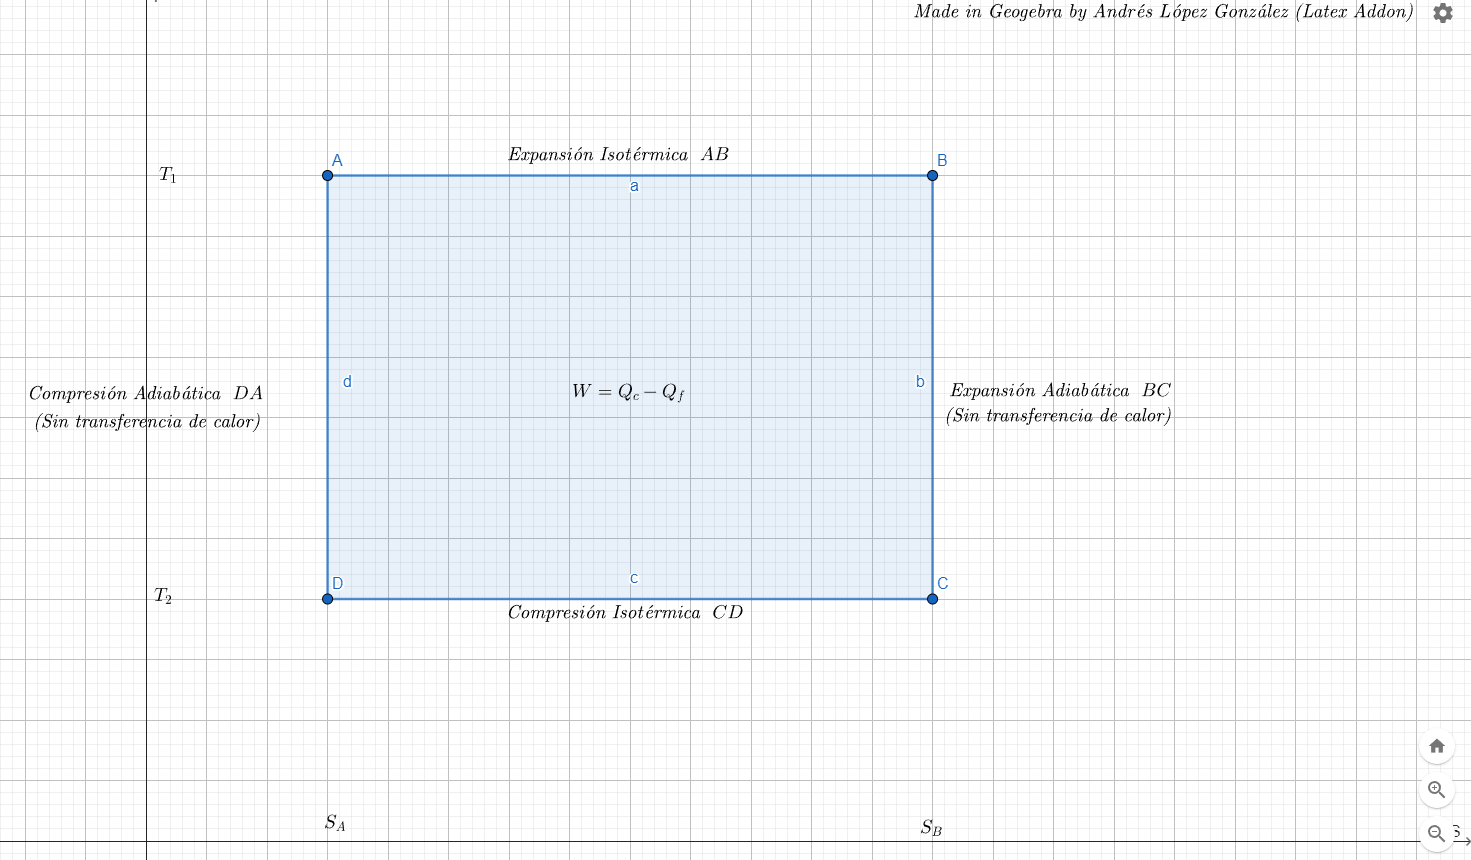
\includegraphics[width=1\linewidth]{Carnot Cycle.png}
    \caption{Carnot Cycle (Temperature vs Entropy)}
    \label{fig:enter-label}
\end{figure}

\end{document}